\documentclass[tikz,border=4pt]{standalone}
\usepackage{amsmath}
\usetikzlibrary{calc}
\begin{document}
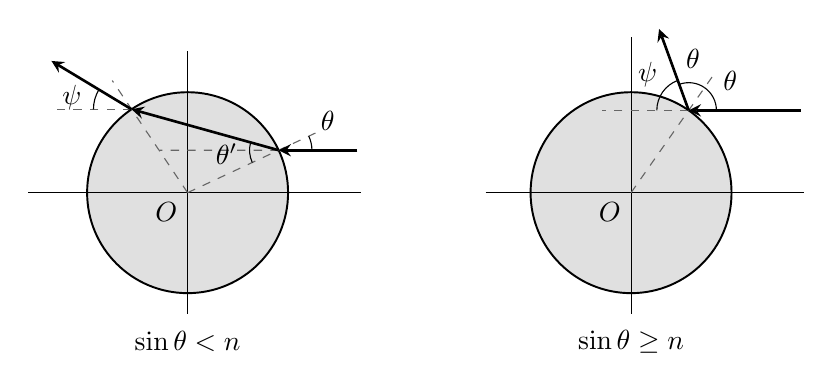
\begin{tikzpicture}[>=stealth, thick, scale=0.88]
  % Left: Refraction (sin theta < n)
  \begin{scope}[xshift=-3.3cm]
    \def\R{1.45}
    \fill[black!12] (0, 0) circle (\R);
    \draw[line width=0.7pt] (0, 0) circle (\R);
    \draw[line width=0.4pt] (-2.3, 0) -- (2.5, 0);
    \draw[line width=0.4pt] (0, -1.75) -- (0, 2.05);
    \node[below left] at (0, 0) {$O$};

    \coordinate (A) at (25:\R);
    \coordinate (B) at (123.9:\R);
    \coordinate (In) at (2.45, {\R*sin(25)});
    \coordinate (Out) at ($(B) + (148.9:1.35)$);

    % Normals
    \draw[dashed, line width=0.4pt, black!60] (0, 0) -- (25:2.15);
    \draw[dashed, line width=0.4pt, black!60] (0, 0) -- (123.9:1.95);

    % Incident extension & outgoing direction for psi
    \draw[dashed, line width=0.4pt, black!60] (A) -- (-0.4, {\R*sin(25)});
    \draw[dashed, line width=0.4pt, black!60] (B) -- ($(B) + (180:1.15)$);

    % Path
    \draw[->, line width=0.95pt] (In) -- (A);
    \draw[->, line width=0.95pt] (A) -- (B);
    \draw[->, line width=0.95pt] (B) -- (Out);

    % Angle theta at A (placed above the normal arc to avoid touching horizontal ray)
    \draw[line width=0.4pt] (A) ++(0:0.48) arc (0:25:0.48);
    \node[above right] at ($(A)+(16:0.48)$) {$\theta$};

    % Angle theta' inside at A
    \draw[line width=0.4pt] (A) ++(164.45:0.42) arc (164.45:205:0.42);
    \node[left] at ($(A)+(188:0.45)$) {$\theta'$};

    % Scattering angle psi at B
    \draw[line width=0.4pt] (B) ++(148.9:0.55) arc (148.9:180:0.55);
    \node[left] at ($(B)+(164:0.60)$) {$\psi$};

    \node at (0, -2.15) {$\sin\theta < n$};
  \end{scope}

  % Right: Total reflection (sin theta >= n)
  \begin{scope}[xshift=3.1cm]
    \def\R{1.45}
    \fill[black!12] (0, 0) circle (\R);
    \draw[line width=0.7pt] (0, 0) circle (\R);
    \draw[line width=0.4pt] (-2.1, 0) -- (2.5, 0);
    \draw[line width=0.4pt] (0, -1.75) -- (0, 2.25);
    \node[below left] at (0, 0) {$O$};

    \coordinate (A) at (55:\R);
    \coordinate (In) at (2.45, {\R*sin(55)});
    \coordinate (Out) at ($(A) + (110:1.25)$);

    % Normal at A
    \draw[dashed, line width=0.4pt, black!60] (0, 0) -- (55:2.05);
    % Extension of incoming ray (-x)
    \draw[dashed, line width=0.4pt, black!60] (A) -- ($(A) + (180:1.25)$);

    % Path
    \draw[->, line width=0.95pt] (In) -- (A);
    \draw[->, line width=0.95pt] (A) -- (Out);

    % Angle theta (between +x and normal)
    \draw[line width=0.4pt] (A) ++(0:0.40) arc (0:55:0.40);
    \node[above right] at ($(A)+(22:0.38)$) {$\theta$};
    % Reflected angle theta
    \draw[line width=0.4pt] (A) ++(55:0.40) arc (55:110:0.40);
    \node[above] at ($(A)+(82:0.46)$) {$\theta$};
    % Scattering angle psi (placed clearly to the right of y-axis)
    \draw[line width=0.4pt] (A) ++(110:0.46) arc (110:180:0.46);
    \node[above left] at ($(A)+(148:0.36)$) {$\psi$};

    \node at (0, -2.15) {$\sin\theta \ge n$};
  \end{scope}
\end{tikzpicture}
\end{document}
